\iffalse
\chapter{2012}
\author{EE24BTECH11059}
\section{xe}
\fi
    %code by ysiddhanth 
	\item{
		Consider two functions
		\( f(z) = z \)
		and
		\( g(z) = \bar{z} \)
		(conjugate of \( z \)). Using Cauchy-Riemann conditions, choose the correct answer
		
		\begin{multicols}{2}
			\begin{enumerate}
				\item Both \(f\) and \(g\) are analytic
				\item \(f\) is analytic but \(g\) is not analytic
				\item \(g\) is analytic but \(f\) is not analytic
				\item Neither \(f\) nor \(g\) is analytic 
			\end{enumerate}
		\end{multicols}
	}
   	\item{
    	For $f\brak{x} = x^4 - 5xy^2 $ the direction of maximum increase of \( f\brak{x,y} \) at the point \( \brak{2,2} \) is along \text{  }\hfill
    	
    	\begin{multicols}{4}
    		\begin{enumerate}
    			\item \(3\hat{i} + 10\hat{j}\)
    			
    			\item \(-12\hat{i} - 40\hat{j}\)
    			
    			\item \(3\hat{i} - 10\hat{j}\)
    			
    			\item \(-12\hat{i} + 40\hat{j}\)
    		\end{enumerate}
    	\end{multicols}
    }
    \item{
            Suppose 50\% of the population of a village like oranges, 70\% of the population like apples, and 40\% like both. If a person is picked at random who likes at least one of these fruits, what is the probability that the person likes oranges?
                
            \begin{multicols}{4}
                \begin{enumerate}
                	\item \( \frac{1}{8} \)
                	\item \( \frac{5}{12} \)
                	\item \( \frac{1}{2} \)
                	\item \( \frac{5}{8} \)
                \end{enumerate}
            \end{multicols}
        }
	\item{
        	
        	For the solution of \(\nabla^2 u = 0\), the domain and boundary conditions are shown below.
        	\hfill
        	\begin{center}
        	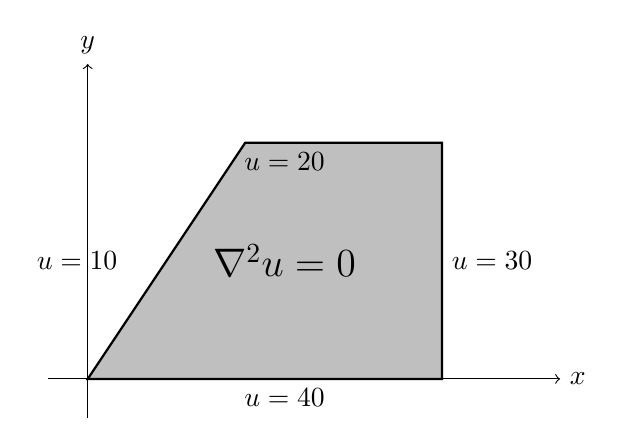
\begin{tikzpicture}
        		% Define points
        		\coordinate (A) at (0,0);       % Bottom-left corner
        		\coordinate (B) at (4.5,0);       % Bottom-right corner
        		\coordinate (C) at (4.5,3);       % Top-right corner
        		\coordinate (D) at (2,3);       % Top-left corner
        		
        		% Draw shaded area
        		\fill[gray!50] (A) -- (B) -- (C) -- (D) -- cycle;
        		
        		% Draw the boundary
        		\draw[thick] (A) -- (B) -- (C) -- (D) -- cycle;
        		
        		% Draw x and y axes
        		\draw[->] (-0.5,0) -- (6,0) node[right] {$x$};
        		\draw[->] (0,-0.5) -- (0,4) node[above] {$y$};
        		
        		% Add boundary conditions
        		\node[anchor=north] at (2.5,3) {$u=20$};
        		\node[anchor=west] at (4.5,1.5) {$u=30$};
        		\node[anchor=north] at (2.5,0) {$u=40$};
        		\node[anchor=east] at (0.5,1.5) {$u=10$};
        		
        		% Add Laplacian symbol
        		\node at (2.5,1.5) {\Large $\nabla^2 u = 0$};
        	\end{tikzpicture}
        \end{center}
        	Which of the following statements is TRUE?
        	\begin{enumerate}
        		\item The solution cannot be obtained using separation of variables because the governing equation is non-separable.
        		\item The solution cannot be obtained using separation of variables because all the boundary values are non-zero.
        		\item The solution cannot be obtained using separation of variables because not all the boundaries are along constant coordinate lines.
        		\item The solution can be obtained by separation of variables.
        	\end{enumerate}
        	
      }
        \item {If \(f\brak{x} = x\sin\brak{x}\) and \(g\brak{x} = |x|\sin(x)\), then
        	
        	\begin{enumerate}
        		\item \(g\brak{x} = |f\brak{x}|\)
        		\item \(g\brak{x}\) is an even function
        		\item The \(x\)-coordinates corresponding to the various local maxima are identical for both \(f\brak{x}\) and \(g\brak{x}\)
        		\item \(g(\brak{x}\) is differentiable at \(x = 0\)
        	\end{enumerate}
  		}
    
    \item {
    	The general solution of $
    	\frac{d^4y}{dx^4} - 2\frac{d^3y}{dx^3} + 2\frac{d^2y}{dx^2} - 2\frac{dy}{dx} + y = 0
    	$
    	is
    	\begin{multicols}{2}
	    	\begin{enumerate}
	    		\item \( c_1 e^x + c_2 xe^x + c_3 \cosh(x) + c_4 \sinh(x) \)
	    		\item \( c_1 e^x + c_2 e^{-x} + c_3 e^{ix} + c_4 e^{-ix} \)
	    		\item \( c_1 e^x + c_2 xe^x + c_3 \cos(x) + c_4 \sin(x) \)
	    		\item \( c_1 e^x + c_2 xe^x + c_3 e^{ix} + c_4 e^{-ix} \)
	    	\end{enumerate}
    	\end{multicols}
    
    }    
    \item {Evaluation of
    	
    	$$
    	\iint_S (e^x\hat{\imath} +3y\hat{\jmath} - ze^x\hat{k})\cdot \hat{n} \, dA
    	$$
    	over a surface \( S : x^2 + y^2 + z^2 = 1 \), using Gauss divergence theorem, gives
    	\begin{multicols}{4}
	    	\begin{enumerate}
	    		\item 0
	    		\item $4\pi$
	    		\item $\frac{4\pi}{3}$
	    		\item $12\pi$
	    	\end{enumerate}
    	\end{multicols}}    
    \item {The exact solution of the integral
    	$$
    	\int_0^4 \brak{x^2-4} \, dx
    	$$
    	is denoted by \( I_E \). The same integral evaluated numerically by the trapezoidal rule and the Simpson’s 1/3 rule are denoted by \( I_T \) and \( I_S \), respectively. The subinterval used in the numerical methods is \( h = 2 \). Then
        \begin{multicols}{2}
	    	\begin{enumerate}
	    		\item \( I_E = I_S > I_T \)
	    		\item \( I_E = I_S < I_T \)
	    		\item \( I_E < I_S < I_T \)
	    		\item \( I_E > I_S > I_T \)
	    	\end{enumerate}
    	\end{multicols}
	}
    \item {
    	In a two-dimensional flow field, the velocities in the $x$- and $y$- directions are $u$ and $v$, respectively. The shear stress for a Newtonian fluid having dynamic viscosity $\mu$ is given by
    	
    	
    	\begin{multicols}{4}
    		\begin{enumerate}
    			\item $
    			\mu \left( \frac{\partial v}{\partial x} - \frac{\partial u}{\partial y} \right)
    			$
    			
    			\item $
    			2\mu \frac{\partial v}{\partial y}
    			$
    			
    			\item $
    			2\mu \frac{\partial u}{\partial x}
    			$
    			
    			\item $
    			\mu \left( \frac{\partial v}{\partial x} + \frac{\partial u}{\partial y} \right)
    			$
    		\end{enumerate}
    	\end{multicols}
    
	}
    \item{
            In a potential flow, the superposition of the stream functions of a uniform flow and a line source gives rise to a dividing streamline representing
            
                
            \begin{multicols}{2}
                \begin{enumerate}
                	\item Rankine’s half-body
                	\item infinite circular cylinder
                	\item infinite rotating circular cylinder
                	\item infinite elliptical cylinder
                \end{enumerate}
            \end{multicols}

        %code by ysiddhanth 
        
        }
    \item{
            Given that \(V\), \(L\), and \(g\) are the characteristic velocity, characteristic length, and acceleration due to gravity, respectively, the expression $
            \frac{V}{\sqrt{Lg}}
            $
            represents
          
            \begin{multicols}{2}
                \begin{enumerate}
                \item Weber number
                \item Euler number
                \item Cavitation number
                \item Froude number
                \end{enumerate}
            \end{multicols}
        
        }
    \item{
            Match the devices in Column I with the characteristics in Column II.
            \begin{tabular}{c@{\hspace{3cm}}c}
	\textbf{Column I} & \textbf{Column II} \\
	P. orifice meter & 1. high head loss and low cost \\
	Q. venturi meter & 2. high head loss and high cost \\
	& 3. low head loss and high cost \\
	& 4. low head loss and low cost \\
\end{tabular}
            \begin{multicols}{4}
				\begin{enumerate}
					\item P - 2; Q - 4
					\item P - 1; Q - 2
					\item P - 3; Q - 1
					\item P - 1; Q - 3
				\end{enumerate}
			\end{multicols}
        }
    \item{
        
           	Identify the visualization method that shows a PATHLINE in an unsteady flow, assuming that the
           	camera covers the required field of view.
				\begin{enumerate}
					\item A dye is continuously injected and a snap shot is taken
					\item A dye is continuously injected and a long-exposure picture is taken
					\item A blob (or drop) of dye is injected and a snap shot is taken
					\item A blob (or drop) of dye is injected and a long-exposure picture is taken
				\end{enumerate}

        
        }


